\section{Практична частина}
\setlength{\parindent}{4em}
\qquad Зменшення сили світла завдяки послаблювачу дорівнює:
$$\frac{I_2}{I_1} = {\frac{r_2}{r_1}}^2 = 10$$
\begin{center}
  {\textbf{\emph{Визначення концентрації розчину за допомогою коефіціента заломлення}}}
\end{center}
\begin{figure}[ht]

\centering

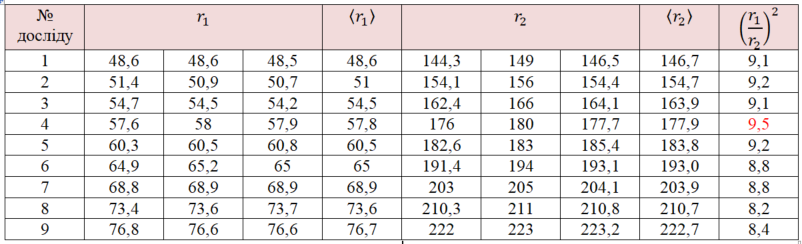
\includegraphics[width=0.55\linewidth]{Pics/tabl1.png}

\label{table1}

\end{figure}
Як видно з розрахунків, найкраще виконується закон обернених квадратів для досліду №4, для якого відношення ${\frac{r_2}{r_1}}^2 = 9,5$, є найбільш точним серед отриманих. \\
Оцінимо при якому відношенні відстані $r_1$ до розмірів джерела закон обернених квадратів виконується найточніше. Розмір джерела: $\Delta = 2 cm$.
$$\frac{r_1}{\Delta} = \frac{57,8}{2} = 23,9$$
\subsection{Визначення кутового розподілу відносної сили світла лампи}
$$I_x = I_0 {\frac{r_x}{r_0}}^2$$
$I_x$ - сила світла лампи, $I_0$ - сила світла еталонної лампи.

\begin{figure}[ht]

\centering

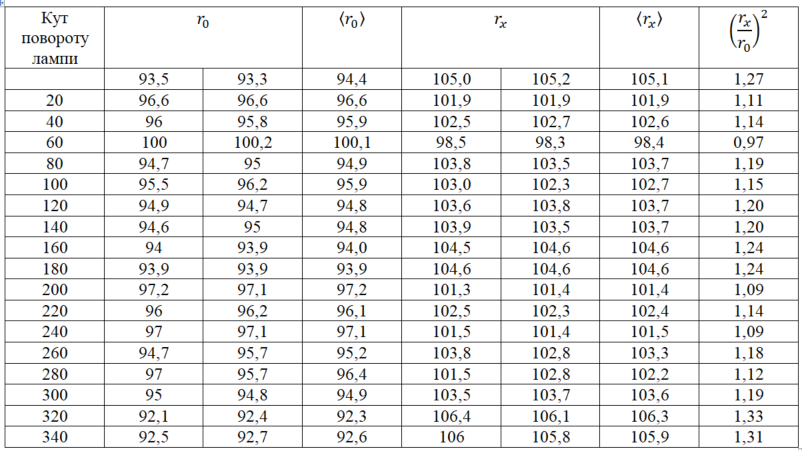
\includegraphics[width=0.7\linewidth]{Pics/tabl2.png}

\label{table1}

\end{figure}

\begin{figure}[ht]

\centering

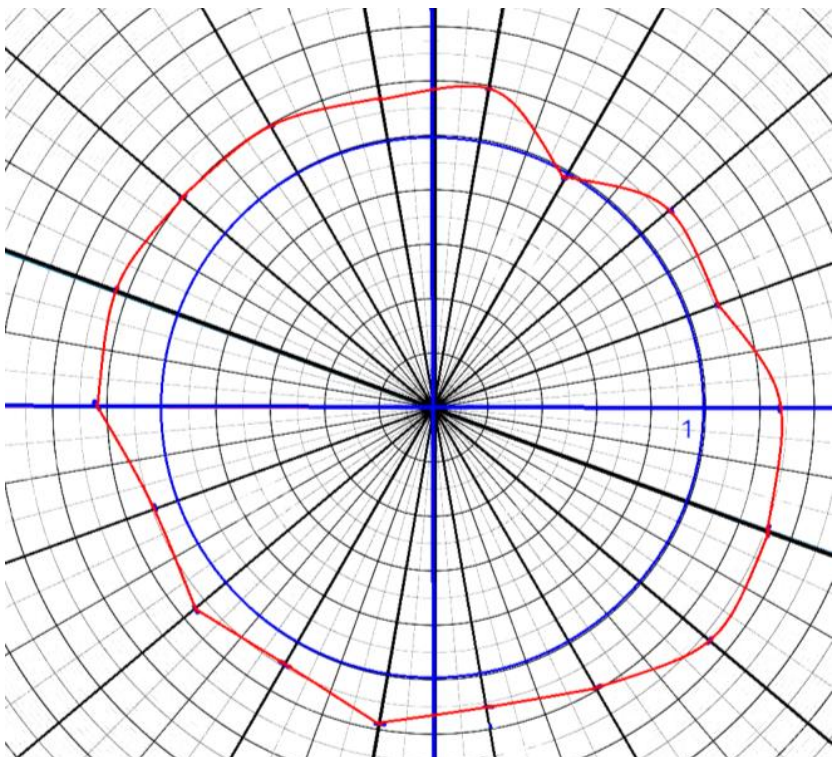
\includegraphics[width=0.7\linewidth]{Pics/tabl3.png}

\label{table1}

\end{figure}

На графіку можна побачити зображення розподілу сила слітла досліджувальної лампи.
